\documentclass[1p]{elsarticle_modified}
%\bibliographystyle{elsarticle-num}

%\usepackage[colorlinks]{hyperref}
%\usepackage{abbrmath_seonhwa} %\Abb, \Ascr, \Acal ,\Abf, \Afrak
\usepackage{amsfonts}
\usepackage{amssymb}
\usepackage{amsmath}
\usepackage{amsthm}
\usepackage{scalefnt}
\usepackage{amsbsy}
\usepackage{kotex}
\usepackage{caption}
\usepackage{subfig}
\usepackage{color}
\usepackage{graphicx}
\usepackage{xcolor} %% white, black, red, green, blue, cyan, magenta, yellow
\usepackage{float}
\usepackage{setspace}
\usepackage{hyperref}

\usepackage{tikz}
\usetikzlibrary{arrows}

\usepackage{multirow}
\usepackage{array} % fixed length table
\usepackage{hhline}

%%%%%%%%%%%%%%%%%%%%%
\makeatletter
\renewcommand*\env@matrix[1][\arraystretch]{%
	\edef\arraystretch{#1}%
	\hskip -\arraycolsep
	\let\@ifnextchar\new@ifnextchar
	\array{*\c@MaxMatrixCols c}}
\makeatother %https://tex.stackexchange.com/questions/14071/how-can-i-increase-the-line-spacing-in-a-matrix
%%%%%%%%%%%%%%%

\usepackage[normalem]{ulem}

\newcommand{\msout}[1]{\ifmmode\text{\sout{\ensuremath{#1}}}\else\sout{#1}\fi}
%SOURCE: \msout is \stkout macro in https://tex.stackexchange.com/questions/20609/strikeout-in-math-mode

\newcommand{\cancel}[1]{
	\ifmmode
	{\color{red}\msout{#1}}
	\else
	{\color{red}\sout{#1}}
	\fi
}

\newcommand{\add}[1]{
	{\color{blue}\uwave{#1}}
}

\newcommand{\replace}[2]{
	\ifmmode
	{\color{red}\msout{#1}}{\color{blue}\uwave{#2}}
	\else
	{\color{red}\sout{#1}}{\color{blue}\uwave{#2}}
	\fi
}

\newcommand{\Sol}{\mathcal{S}} %segment
\newcommand{\D}{D} %diagram
\newcommand{\A}{\mathcal{A}} %arc


%%%%%%%%%%%%%%%%%%%%%%%%%%%%%5 test

\def\sl{\operatorname{\textup{SL}}(2,\Cbb)}
\def\psl{\operatorname{\textup{PSL}}(2,\Cbb)}
\def\quan{\mkern 1mu \triangleright \mkern 1mu}

\theoremstyle{definition}
\newtheorem{thm}{Theorem}[section]
\newtheorem{prop}[thm]{Proposition}
\newtheorem{lem}[thm]{Lemma}
\newtheorem{ques}[thm]{Question}
\newtheorem{cor}[thm]{Corollary}
\newtheorem{defn}[thm]{Definition}
\newtheorem{exam}[thm]{Example}
\newtheorem{rmk}[thm]{Remark}
\newtheorem{alg}[thm]{Algorithm}

\newcommand{\I}{\sqrt{-1}}
\begin{document}

%\begin{frontmatter}
%
%\title{Boundary parabolic representations of knots up to 8 crossings}
%
%%% Group authors per affiliation:
%\author{Yunhi Cho} 
%\address{Department of Mathematics, University of Seoul, Seoul, Korea}
%\ead{yhcho@uos.ac.kr}
%
%
%\author{Seonhwa Kim} %\fnref{s_kim}}
%\address{Center for Geometry and Physics, Institute for Basic Science, Pohang, 37673, Korea}
%\ead{ryeona17@ibs.re.kr}
%
%\author{Hyuk Kim}
%\address{Department of Mathematical Sciences, Seoul National University, Seoul 08826, Korea}
%\ead{hyukkim@snu.ac.kr}
%
%\author{Seokbeom Yoon}
%\address{Department of Mathematical Sciences, Seoul National University, Seoul, 08826,  Korea}
%\ead{sbyoon15@snu.ac.kr}
%
%\begin{abstract}
%We find all boundary parabolic representation of knots up to 8 crossings.
%
%\end{abstract}
%\begin{keyword}
%    \MSC[2010] 57M25 
%\end{keyword}
%
%\end{frontmatter}

%\linenumbers
%\tableofcontents
%
\newcommand\colored[1]{\textcolor{white}{\rule[-0.35ex]{0.8em}{1.4ex}}\kern-0.8em\color{red} #1}%
%\newcommand\colored[1]{\textcolor{white}{ #1}\kern-2.17ex	\textcolor{white}{ #1}\kern-1.81ex	\textcolor{white}{ #1}\kern-2.15ex\color{red}#1	}

{\Large $\underline{12n_{0520}~(K12n_{0520})}$}

\setlength{\tabcolsep}{10pt}
\renewcommand{\arraystretch}{1.6}
\vspace{1cm}\begin{tabular}{m{100pt}>{\centering\arraybackslash}m{274pt}}
\multirow{5}{120pt}{
	\centering
	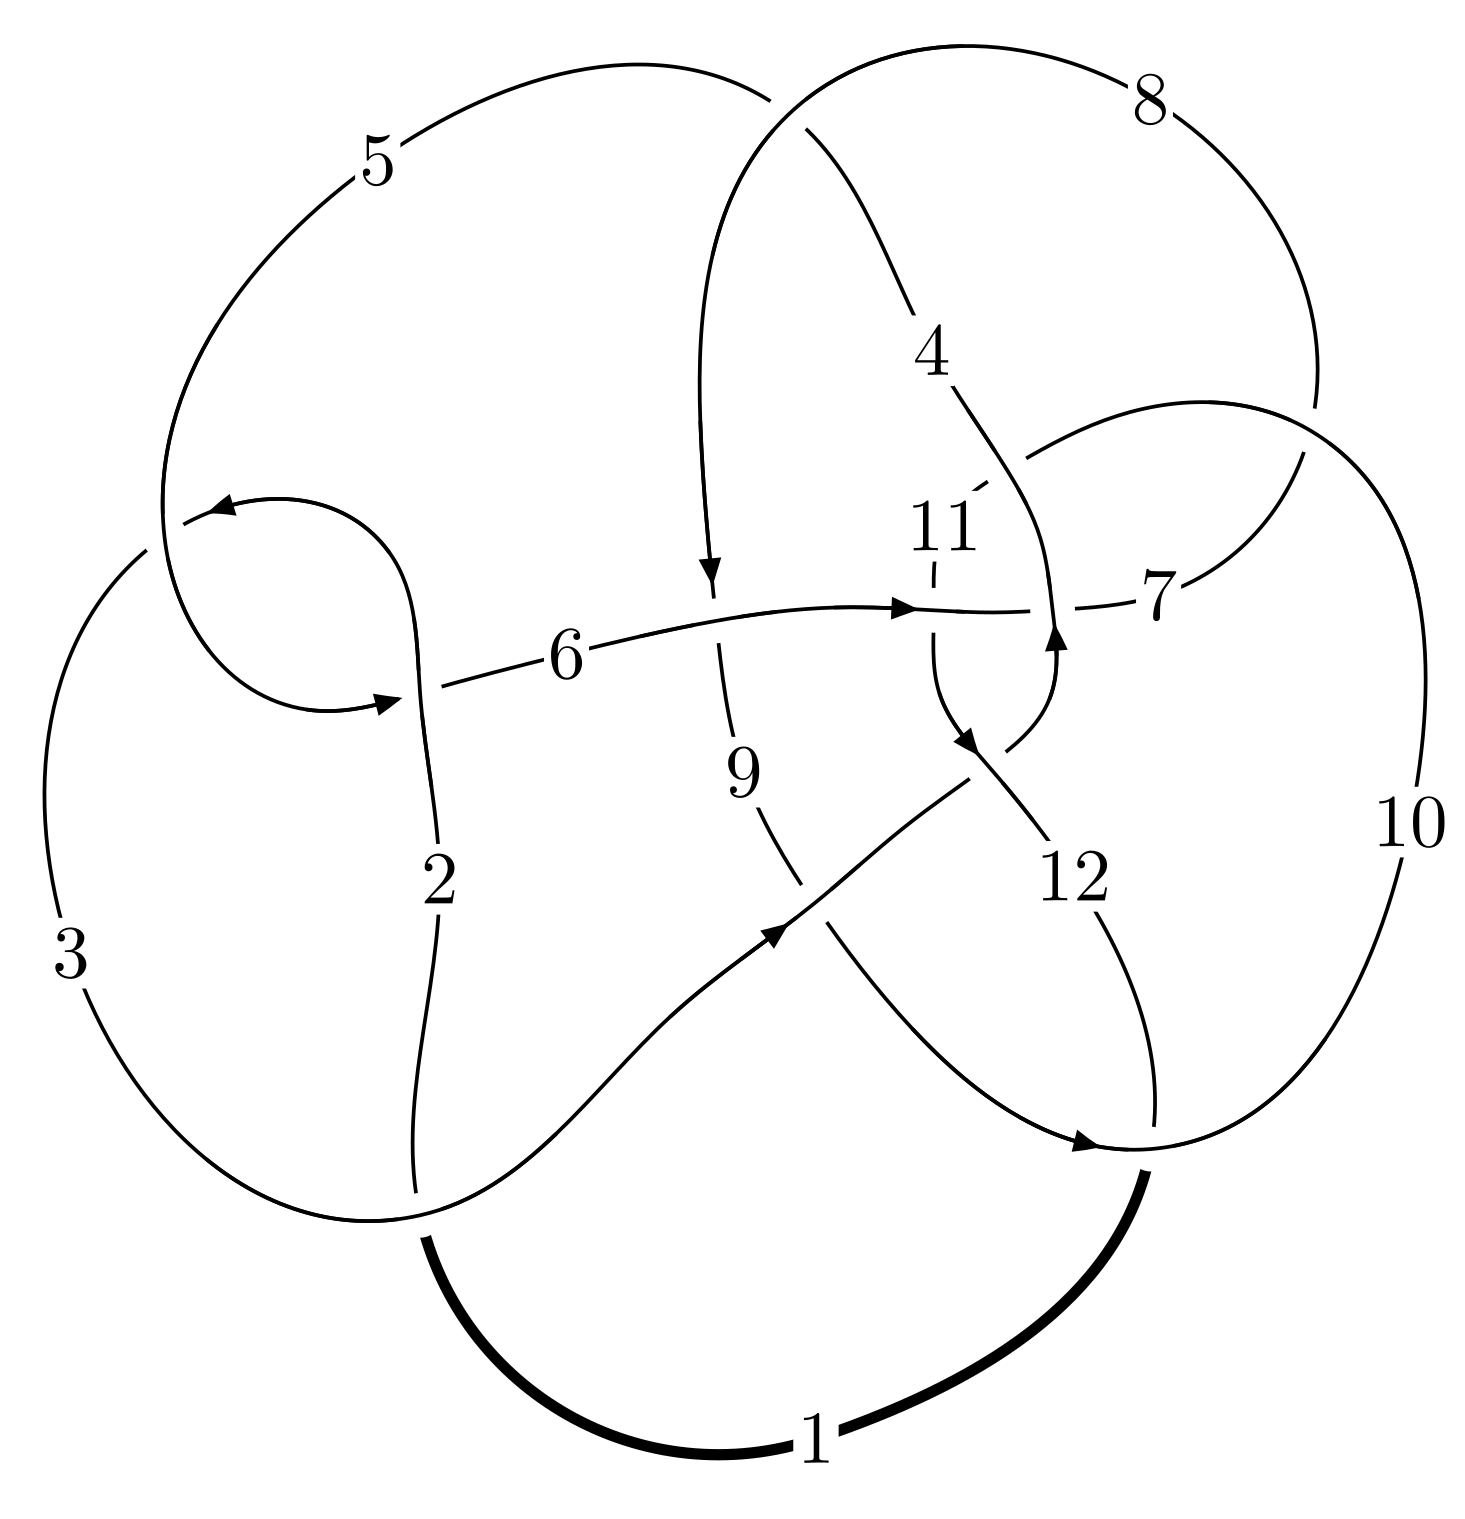
\includegraphics[width=112pt]{../../../GIT/diagram.site/Diagrams/png/2609_12n_0520.png}\\
\ \ \ A knot diagram\footnotemark}&
\allowdisplaybreaks
\textbf{Linearized knot diagam} \\
\cline{2-2}
 &
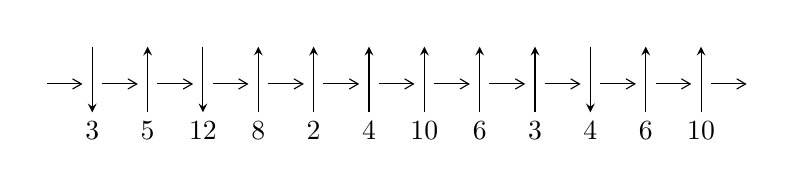
\begin{tikzpicture}[x=20pt, y=17pt]
	% nodes
	\node (C0) at (0, 0) {};
	\node (C1) at (1, 0) {};
	\node (C1U) at (1, +1) {};
	\node (C1D) at (1, -1) {3};

	\node (C2) at (2, 0) {};
	\node (C2U) at (2, +1) {};
	\node (C2D) at (2, -1) {5};

	\node (C3) at (3, 0) {};
	\node (C3U) at (3, +1) {};
	\node (C3D) at (3, -1) {12};

	\node (C4) at (4, 0) {};
	\node (C4U) at (4, +1) {};
	\node (C4D) at (4, -1) {8};

	\node (C5) at (5, 0) {};
	\node (C5U) at (5, +1) {};
	\node (C5D) at (5, -1) {2};

	\node (C6) at (6, 0) {};
	\node (C6U) at (6, +1) {};
	\node (C6D) at (6, -1) {4};

	\node (C7) at (7, 0) {};
	\node (C7U) at (7, +1) {};
	\node (C7D) at (7, -1) {10};

	\node (C8) at (8, 0) {};
	\node (C8U) at (8, +1) {};
	\node (C8D) at (8, -1) {6};

	\node (C9) at (9, 0) {};
	\node (C9U) at (9, +1) {};
	\node (C9D) at (9, -1) {3};

	\node (C10) at (10, 0) {};
	\node (C10U) at (10, +1) {};
	\node (C10D) at (10, -1) {4};

	\node (C11) at (11, 0) {};
	\node (C11U) at (11, +1) {};
	\node (C11D) at (11, -1) {6};

	\node (C12) at (12, 0) {};
	\node (C12U) at (12, +1) {};
	\node (C12D) at (12, -1) {10};
	\node (C13) at (13, 0) {};

	% arrows
	\draw[->,>={angle 60}]
	(C0) edge (C1) (C1) edge (C2) (C2) edge (C3) (C3) edge (C4) (C4) edge (C5) (C5) edge (C6) (C6) edge (C7) (C7) edge (C8) (C8) edge (C9) (C9) edge (C10) (C10) edge (C11) (C11) edge (C12) (C12) edge (C13) ;	\draw[->,>=stealth]
	(C1U) edge (C1D) (C2D) edge (C2U) (C3U) edge (C3D) (C4D) edge (C4U) (C5D) edge (C5U) (C6D) edge (C6U) (C7D) edge (C7U) (C8D) edge (C8U) (C9D) edge (C9U) (C10U) edge (C10D) (C11D) edge (C11U) (C12D) edge (C12U) ;
	\end{tikzpicture} \\
\hhline{~~} \\& 
\textbf{Solving Sequence} \\ \cline{2-2} 
 &
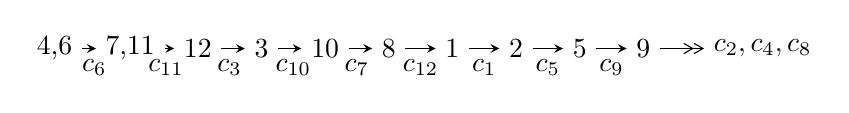
\begin{tikzpicture}[x=23pt, y=7pt]
	% node
	\node (A0) at (-1/8, 0) {4,6};
	\node (A1) at (17/16, 0) {7,11};
	\node (A2) at (17/8, 0) {12};
	\node (A3) at (25/8, 0) {3};
	\node (A4) at (33/8, 0) {10};
	\node (A5) at (41/8, 0) {8};
	\node (A6) at (49/8, 0) {1};
	\node (A7) at (57/8, 0) {2};
	\node (A8) at (65/8, 0) {5};
	\node (A9) at (73/8, 0) {9};
	\node (C1) at (1/2, -1) {$c_{6}$};
	\node (C2) at (13/8, -1) {$c_{11}$};
	\node (C3) at (21/8, -1) {$c_{3}$};
	\node (C4) at (29/8, -1) {$c_{10}$};
	\node (C5) at (37/8, -1) {$c_{7}$};
	\node (C6) at (45/8, -1) {$c_{12}$};
	\node (C7) at (53/8, -1) {$c_{1}$};
	\node (C8) at (61/8, -1) {$c_{5}$};
	\node (C9) at (69/8, -1) {$c_{9}$};
	\node (A10) at (11, 0) {$c_{2},c_{4},c_{8}$};

	% edge
	\draw[->,>=stealth]	
	(A0) edge (A1) (A1) edge (A2) (A2) edge (A3) (A3) edge (A4) (A4) edge (A5) (A5) edge (A6) (A6) edge (A7) (A7) edge (A8) (A8) edge (A9) ;
	\draw[->>,>={angle 60}]	
	(A9) edge (A10);
\end{tikzpicture} \\ 

\end{tabular} \\

\footnotetext{
The image of knot diagram is generated by the software ``\textbf{Draw programme}" developed by Andrew Bartholomew(\url{http://www.layer8.co.uk/maths/draw/index.htm\#Running-draw}), where we modified some parts for our purpose(\url{https://github.com/CATsTAILs/LinksPainter}).
}\phantom \\ \newline 
\centering \textbf{Ideals for irreducible components\footnotemark of $X_{\text{par}}$} 
 
\begin{align*}
I^u_{1}&=\langle 
-1.00773\times10^{215} u^{54}+3.95891\times10^{215} u^{53}+\cdots+5.25110\times10^{219} b-1.48407\times10^{220},\\
\phantom{I^u_{1}}&\phantom{= \langle  }-1.77810\times10^{217} u^{54}-8.41460\times10^{217} u^{53}+\cdots+1.78060\times10^{221} a+4.35856\times10^{221},\\
\phantom{I^u_{1}}&\phantom{= \langle  }u^{55}+3 u^{54}+\cdots+4862 u-6341\rangle \\
I^u_{2}&=\langle 
9.41498\times10^{23} u^{19}+2.05689\times10^{24} u^{18}+\cdots+9.99999\times10^{23} b-4.03582\times10^{24},\\
\phantom{I^u_{2}}&\phantom{= \langle  }3.23988\times10^{25} u^{19}+7.09015\times10^{25} u^{18}+\cdots+9.99999\times10^{23} a-1.70850\times10^{26},\;u^{20}+2 u^{19}+\cdots-14 u+1\rangle \\
\\
\end{align*}
\raggedright * 2 irreducible components of $\dim_{\mathbb{C}}=0$, with total 75 representations.\\
\footnotetext{All coefficients of polynomials are rational numbers. But the coefficients are sometimes approximated in decimal forms when there is not enough margin.}
\newpage
\renewcommand{\arraystretch}{1}
\centering \section*{I. $I^u_{1}= \langle -1.01\times10^{215} u^{54}+3.96\times10^{215} u^{53}+\cdots+5.25\times10^{219} b-1.48\times10^{220},\;-1.78\times10^{217} u^{54}-8.41\times10^{217} u^{53}+\cdots+1.78\times10^{221} a+4.36\times10^{221},\;u^{55}+3 u^{54}+\cdots+4862 u-6341 \rangle$}
\flushleft \textbf{(i) Arc colorings}\\
\begin{tabular}{m{7pt} m{180pt} m{7pt} m{180pt} }
\flushright $a_{4}=$&$\begin{pmatrix}0\\u\end{pmatrix}$ \\
\flushright $a_{6}=$&$\begin{pmatrix}1\\0\end{pmatrix}$ \\
\flushright $a_{7}=$&$\begin{pmatrix}1\\- u^2\end{pmatrix}$ \\
\flushright $a_{11}=$&$\begin{pmatrix}0.0000998597 u^{54}+0.000472571 u^{53}+\cdots-1.70493 u-2.44781\\0.0000191908 u^{54}-0.0000753920 u^{53}+\cdots+2.51058 u+2.82621\end{pmatrix}$ \\
\flushright $a_{12}=$&$\begin{pmatrix}0.000119051 u^{54}+0.000397179 u^{53}+\cdots+0.805651 u+0.378407\\0.0000191908 u^{54}-0.0000753920 u^{53}+\cdots+2.51058 u+2.82621\end{pmatrix}$ \\
\flushright $a_{3}=$&$\begin{pmatrix}0.000439453 u^{54}+0.00130155 u^{53}+\cdots-9.12833 u+2.22261\\5.39110\times10^{-6} u^{54}-0.0000762385 u^{53}+\cdots+0.556271 u+2.93121\end{pmatrix}$ \\
\flushright $a_{10}=$&$\begin{pmatrix}0.0000998597 u^{54}+0.000472571 u^{53}+\cdots-1.70493 u-2.44781\\0.0000160377 u^{54}-0.0000345076 u^{53}+\cdots+2.71846 u+1.72927\end{pmatrix}$ \\
\flushright $a_{8}=$&$\begin{pmatrix}-0.0000108886 u^{54}-0.0000519635 u^{53}+\cdots-1.50476 u+0.832419\\-0.000450416 u^{54}-0.00135705 u^{53}+\cdots+13.8133 u-1.51385\end{pmatrix}$ \\
\flushright $a_{1}=$&$\begin{pmatrix}8.14406\times10^{-8} u^{54}-0.000279970 u^{53}+\cdots+6.32497 u+7.75382\\-0.000125932 u^{54}-0.000589665 u^{53}+\cdots+3.03504 u+3.45260\end{pmatrix}$ \\
\flushright $a_{2}=$&$\begin{pmatrix}-0.0000620439 u^{54}-0.000144711 u^{53}+\cdots+3.04412 u+0.737987\\0.000267626 u^{54}+0.000799507 u^{53}+\cdots-8.68003 u+0.274355\end{pmatrix}$ \\
\flushright $a_{5}=$&$\begin{pmatrix}0.000100081 u^{54}+0.000476708 u^{53}+\cdots-2.36634 u-2.92983\\0.000135989 u^{54}+0.000606267 u^{53}+\cdots-0.718613 u-4.76962\end{pmatrix}$ \\
\flushright $a_{9}=$&$\begin{pmatrix}-0.000461305 u^{54}-0.00140901 u^{53}+\cdots+12.3085 u-0.681429\\-0.000450416 u^{54}-0.00135705 u^{53}+\cdots+13.8133 u-1.51385\end{pmatrix}$\\&\end{tabular}
\flushleft \textbf{(ii) Obstruction class $= -1$}\\~\\
\flushleft \textbf{(iii) Cusp Shapes $= -0.00197309 u^{54}-0.00651879 u^{53}+\cdots+43.1168 u+3.92550$}\\~\\
\newpage\renewcommand{\arraystretch}{1}
\flushleft \textbf{(iv) u-Polynomials at the component}\newline \\
\begin{tabular}{m{50pt}|m{274pt}}
Crossings & \hspace{64pt}u-Polynomials at each crossing \\
\hline $$\begin{aligned}c_{1}\end{aligned}$$&$\begin{aligned}
&u^{55}+34 u^{54}+\cdots+261 u-169
\end{aligned}$\\
\hline $$\begin{aligned}c_{2},c_{5}\end{aligned}$$&$\begin{aligned}
&u^{55}+17 u^{53}+\cdots- u-13
\end{aligned}$\\
\hline $$\begin{aligned}c_{3}\end{aligned}$$&$\begin{aligned}
&u^{55}-4 u^{54}+\cdots-29 u-1
\end{aligned}$\\
\hline $$\begin{aligned}c_{4}\end{aligned}$$&$\begin{aligned}
&u^{55}-3 u^{54}+\cdots-160 u-29
\end{aligned}$\\
\hline $$\begin{aligned}c_{6}\end{aligned}$$&$\begin{aligned}
&u^{55}+3 u^{54}+\cdots+4862 u-6341
\end{aligned}$\\
\hline $$\begin{aligned}c_{7},c_{11}\end{aligned}$$&$\begin{aligned}
&u^{55}+u^{54}+\cdots+1301 u-319
\end{aligned}$\\
\hline $$\begin{aligned}c_{8}\end{aligned}$$&$\begin{aligned}
&u^{55}+9 u^{54}+\cdots-23423 u-2897
\end{aligned}$\\
\hline $$\begin{aligned}c_{9}\end{aligned}$$&$\begin{aligned}
&u^{55}-2 u^{54}+\cdots-8637 u-2059
\end{aligned}$\\
\hline $$\begin{aligned}c_{10}\end{aligned}$$&$\begin{aligned}
&u^{55}+2 u^{54}+\cdots+31739 u-6187
\end{aligned}$\\
\hline $$\begin{aligned}c_{12}\end{aligned}$$&$\begin{aligned}
&u^{55}+4 u^{54}+\cdots+5373 u-431
\end{aligned}$\\
\hline
\end{tabular}\\~\\
\newpage\renewcommand{\arraystretch}{1}
\flushleft \textbf{(v) Riley Polynomials at the component}\newline \\
\begin{tabular}{m{50pt}|m{274pt}}
Crossings & \hspace{64pt}Riley Polynomials at each crossing \\
\hline $$\begin{aligned}c_{1}\end{aligned}$$&$\begin{aligned}
&y^{55}-18 y^{54}+\cdots+2763333 y-28561
\end{aligned}$\\
\hline $$\begin{aligned}c_{2},c_{5}\end{aligned}$$&$\begin{aligned}
&y^{55}+34 y^{54}+\cdots+261 y-169
\end{aligned}$\\
\hline $$\begin{aligned}c_{3}\end{aligned}$$&$\begin{aligned}
&y^{55}-6 y^{54}+\cdots+581 y-1
\end{aligned}$\\
\hline $$\begin{aligned}c_{4}\end{aligned}$$&$\begin{aligned}
&y^{55}-5 y^{54}+\cdots-35184 y-841
\end{aligned}$\\
\hline $$\begin{aligned}c_{6}\end{aligned}$$&$\begin{aligned}
&y^{55}+73 y^{54}+\cdots-1088711858 y-40208281
\end{aligned}$\\
\hline $$\begin{aligned}c_{7},c_{11}\end{aligned}$$&$\begin{aligned}
&y^{55}+63 y^{54}+\cdots-2658559 y-101761
\end{aligned}$\\
\hline $$\begin{aligned}c_{8}\end{aligned}$$&$\begin{aligned}
&y^{55}+35 y^{54}+\cdots-164702969 y-8392609
\end{aligned}$\\
\hline $$\begin{aligned}c_{9}\end{aligned}$$&$\begin{aligned}
&y^{55}+62 y^{54}+\cdots-51063001 y-4239481
\end{aligned}$\\
\hline $$\begin{aligned}c_{10}\end{aligned}$$&$\begin{aligned}
&y^{55}-68 y^{54}+\cdots+631132651 y-38278969
\end{aligned}$\\
\hline $$\begin{aligned}c_{12}\end{aligned}$$&$\begin{aligned}
&y^{55}+50 y^{54}+\cdots+5965789 y-185761
\end{aligned}$\\
\hline
\end{tabular}\\~\\
\newpage\flushleft \textbf{(vi) Complex Volumes and Cusp Shapes}
$$\begin{array}{c|c|c}  
\text{Solutions to }I^u_{1}& \I (\text{vol} + \sqrt{-1}CS) & \text{Cusp shape}\\
 \hline 
\begin{aligned}
u &= \phantom{-}0.458700 + 0.836212 I \\
a &= \phantom{-}0.47157 + 1.49663 I \\
b &= \phantom{-}0.305132 - 0.747908 I\end{aligned}
 & \phantom{-}0.11183 + 1.55303 I & \phantom{-}1.95072 - 2.89152 I \\ \hline\begin{aligned}
u &= \phantom{-}0.458700 - 0.836212 I \\
a &= \phantom{-}0.47157 - 1.49663 I \\
b &= \phantom{-}0.305132 + 0.747908 I\end{aligned}
 & \phantom{-}0.11183 - 1.55303 I & \phantom{-}1.95072 + 2.89152 I \\ \hline\begin{aligned}
u &= \phantom{-}0.913175 + 0.260802 I \\
a &= -0.223977 - 0.423038 I \\
b &= -0.550856 - 0.738530 I\end{aligned}
 & \phantom{-}3.80751 - 0.71144 I & \phantom{-}10.81195 - 1.56897 I \\ \hline\begin{aligned}
u &= \phantom{-}0.913175 - 0.260802 I \\
a &= -0.223977 + 0.423038 I \\
b &= -0.550856 + 0.738530 I\end{aligned}
 & \phantom{-}3.80751 + 0.71144 I & \phantom{-}10.81195 + 1.56897 I \\ \hline\begin{aligned}
u &= -1.113670 + 0.091899 I \\
a &= -0.65683 + 1.51641 I \\
b &= \phantom{-}0.111069 - 0.811383 I\end{aligned}
 & -5.06254 + 5.92628 I & \phantom{-0.000000 } 0. - 4.32930 I \\ \hline\begin{aligned}
u &= -1.113670 - 0.091899 I \\
a &= -0.65683 - 1.51641 I \\
b &= \phantom{-}0.111069 + 0.811383 I\end{aligned}
 & -5.06254 - 5.92628 I & \phantom{-0.000000 -}0. + 4.32930 I \\ \hline\begin{aligned}
u &= \phantom{-}0.797854 + 0.338507 I \\
a &= \phantom{-}1.240170 + 0.296206 I \\
b &= -0.473741 + 0.512242 I\end{aligned}
 & \phantom{-}0.29315 - 1.97385 I & \phantom{-}5.19969 + 3.03837 I \\ \hline\begin{aligned}
u &= \phantom{-}0.797854 - 0.338507 I \\
a &= \phantom{-}1.240170 - 0.296206 I \\
b &= -0.473741 - 0.512242 I\end{aligned}
 & \phantom{-}0.29315 + 1.97385 I & \phantom{-}5.19969 - 3.03837 I \\ \hline\begin{aligned}
u &= -0.591324 + 0.479194 I \\
a &= -0.793327 + 0.649542 I \\
b &= -0.407085 + 0.865255 I\end{aligned}
 & \phantom{-}3.30919 - 4.09772 I & \phantom{-}10.16062 + 6.84746 I \\ \hline\begin{aligned}
u &= -0.591324 - 0.479194 I \\
a &= -0.793327 - 0.649542 I \\
b &= -0.407085 - 0.865255 I\end{aligned}
 & \phantom{-}3.30919 + 4.09772 I & \phantom{-}10.16062 - 6.84746 I\\
 \hline 
 \end{array}$$\newpage$$\begin{array}{c|c|c}  
\text{Solutions to }I^u_{1}& \I (\text{vol} + \sqrt{-1}CS) & \text{Cusp shape}\\
 \hline 
\begin{aligned}
u &= -0.708799 + 0.253071 I \\
a &= \phantom{-}0.831284 + 0.009450 I \\
b &= -0.209759 + 0.509237 I\end{aligned}
 & -1.81477 - 2.14360 I & \phantom{-}1.18374 + 4.80550 I \\ \hline\begin{aligned}
u &= -0.708799 - 0.253071 I \\
a &= \phantom{-}0.831284 - 0.009450 I \\
b &= -0.209759 - 0.509237 I\end{aligned}
 & -1.81477 + 2.14360 I & \phantom{-}1.18374 - 4.80550 I \\ \hline\begin{aligned}
u &= \phantom{-}0.138897 + 0.673640 I \\
a &= \phantom{-}0.011792 - 0.623544 I \\
b &= \phantom{-}0.910818 - 0.785919 I\end{aligned}
 & -7.26057 + 1.21645 I & \phantom{-}0.427980 + 0.554142 I \\ \hline\begin{aligned}
u &= \phantom{-}0.138897 - 0.673640 I \\
a &= \phantom{-}0.011792 + 0.623544 I \\
b &= \phantom{-}0.910818 + 0.785919 I\end{aligned}
 & -7.26057 - 1.21645 I & \phantom{-}0.427980 - 0.554142 I \\ \hline\begin{aligned}
u &= -0.409118 + 0.518801 I \\
a &= \phantom{-}1.81243 - 0.36306 I \\
b &= -0.368450 - 0.362485 I\end{aligned}
 & \phantom{-}0.707490 + 1.043870 I & \phantom{-}2.63060 + 1.21674 I \\ \hline\begin{aligned}
u &= -0.409118 - 0.518801 I \\
a &= \phantom{-}1.81243 + 0.36306 I \\
b &= -0.368450 + 0.362485 I\end{aligned}
 & \phantom{-}0.707490 - 1.043870 I & \phantom{-}2.63060 - 1.21674 I \\ \hline\begin{aligned}
u &= -0.467933 + 1.326800 I \\
a &= \phantom{-}0.355998 + 0.883423 I \\
b &= -0.520534 - 1.220730 I\end{aligned}
 & -2.57844 + 3.79796 I & \phantom{-0.000000 } 0 \\ \hline\begin{aligned}
u &= -0.467933 - 1.326800 I \\
a &= \phantom{-}0.355998 - 0.883423 I \\
b &= -0.520534 + 1.220730 I\end{aligned}
 & -2.57844 - 3.79796 I & \phantom{-0.000000 } 0 \\ \hline\begin{aligned}
u &= -0.177490 + 0.564262 I \\
a &= \phantom{-}0.264895 + 0.985043 I \\
b &= \phantom{-}1.079970 + 0.527227 I\end{aligned}
 & -2.81057 + 3.19886 I & \phantom{-}4.08250 - 3.76051 I \\ \hline\begin{aligned}
u &= -0.177490 - 0.564262 I \\
a &= \phantom{-}0.264895 - 0.985043 I \\
b &= \phantom{-}1.079970 - 0.527227 I\end{aligned}
 & -2.81057 - 3.19886 I & \phantom{-}4.08250 + 3.76051 I\\
 \hline 
 \end{array}$$\newpage$$\begin{array}{c|c|c}  
\text{Solutions to }I^u_{1}& \I (\text{vol} + \sqrt{-1}CS) & \text{Cusp shape}\\
 \hline 
\begin{aligned}
u &= \phantom{-}0.122496 + 0.504032 I \\
a &= \phantom{-}0.083451 - 1.312890 I \\
b &= \phantom{-}1.280030 - 0.596135 I\end{aligned}
 & -6.14972 - 8.50203 I & \phantom{-}1.50480 + 6.85692 I \\ \hline\begin{aligned}
u &= \phantom{-}0.122496 - 0.504032 I \\
a &= \phantom{-}0.083451 + 1.312890 I \\
b &= \phantom{-}1.280030 + 0.596135 I\end{aligned}
 & -6.14972 + 8.50203 I & \phantom{-}1.50480 - 6.85692 I \\ \hline\begin{aligned}
u &= -0.038547 + 0.511598 I \\
a &= \phantom{-}1.50581 + 0.77163 I \\
b &= \phantom{-}0.185020 - 0.254061 I\end{aligned}
 & \phantom{-}0.38570 + 1.60336 I & \phantom{-}2.33296 - 4.99216 I \\ \hline\begin{aligned}
u &= -0.038547 - 0.511598 I \\
a &= \phantom{-}1.50581 - 0.77163 I \\
b &= \phantom{-}0.185020 + 0.254061 I\end{aligned}
 & \phantom{-}0.38570 - 1.60336 I & \phantom{-}2.33296 + 4.99216 I \\ \hline\begin{aligned}
u &= \phantom{-}0.454497\phantom{ +0.000000I} \\
a &= \phantom{-}0.867401\phantom{ +0.000000I} \\
b &= -0.487142\phantom{ +0.000000I}\end{aligned}
 & \phantom{-}0.882935\phantom{ +0.000000I} & \phantom{-}11.1550\phantom{ +0.000000I} \\ \hline\begin{aligned}
u &= -0.35658 + 1.53590 I \\
a &= -0.006681 - 1.169070 I \\
b &= -0.22183 + 1.78303 I\end{aligned}
 & -7.14735 - 6.72459 I & \phantom{-0.000000 } 0 \\ \hline\begin{aligned}
u &= -0.35658 - 1.53590 I \\
a &= -0.006681 + 1.169070 I \\
b &= -0.22183 - 1.78303 I\end{aligned}
 & -7.14735 + 6.72459 I & \phantom{-0.000000 } 0 \\ \hline\begin{aligned}
u &= \phantom{-}1.32120 + 0.87148 I \\
a &= \phantom{-}0.072899 - 0.543533 I \\
b &= -0.362960 + 0.792328 I\end{aligned}
 & -0.103767 + 0.867284 I & \phantom{-0.000000 } 0 \\ \hline\begin{aligned}
u &= \phantom{-}1.32120 - 0.87148 I \\
a &= \phantom{-}0.072899 + 0.543533 I \\
b &= -0.362960 - 0.792328 I\end{aligned}
 & -0.103767 - 0.867284 I & \phantom{-0.000000 } 0 \\ \hline\begin{aligned}
u &= \phantom{-}0.150297 + 0.353433 I \\
a &= \phantom{-}1.088790 - 0.154193 I \\
b &= -1.184760 + 0.246323 I\end{aligned}
 & \phantom{-}1.04688 - 1.12802 I & -3.55524 - 3.81322 I\\
 \hline 
 \end{array}$$\newpage$$\begin{array}{c|c|c}  
\text{Solutions to }I^u_{1}& \I (\text{vol} + \sqrt{-1}CS) & \text{Cusp shape}\\
 \hline 
\begin{aligned}
u &= \phantom{-}0.150297 - 0.353433 I \\
a &= \phantom{-}1.088790 + 0.154193 I \\
b &= -1.184760 - 0.246323 I\end{aligned}
 & \phantom{-}1.04688 + 1.12802 I & -3.55524 + 3.81322 I \\ \hline\begin{aligned}
u &= \phantom{-}0.19519 + 1.66111 I \\
a &= \phantom{-}0.124385 + 1.042830 I \\
b &= -0.23067 - 1.60897 I\end{aligned}
 & -4.50056 + 3.53769 I & \phantom{-0.000000 } 0 \\ \hline\begin{aligned}
u &= \phantom{-}0.19519 - 1.66111 I \\
a &= \phantom{-}0.124385 - 1.042830 I \\
b &= -0.23067 + 1.60897 I\end{aligned}
 & -4.50056 - 3.53769 I & \phantom{-0.000000 } 0 \\ \hline\begin{aligned}
u &= -0.17081 + 1.69824 I \\
a &= \phantom{-}0.260758 - 1.042020 I \\
b &= \phantom{-}0.445170 + 1.129250 I\end{aligned}
 & -1.68388 + 4.70781 I & \phantom{-0.000000 } 0 \\ \hline\begin{aligned}
u &= -0.17081 - 1.69824 I \\
a &= \phantom{-}0.260758 + 1.042020 I \\
b &= \phantom{-}0.445170 - 1.129250 I\end{aligned}
 & -1.68388 - 4.70781 I & \phantom{-0.000000 } 0 \\ \hline\begin{aligned}
u &= -0.37546 + 1.72257 I \\
a &= -0.042439 - 0.816658 I \\
b &= -0.01000 + 1.66318 I\end{aligned}
 & -6.17568 - 1.37212 I & \phantom{-0.000000 } 0 \\ \hline\begin{aligned}
u &= -0.37546 - 1.72257 I \\
a &= -0.042439 + 0.816658 I \\
b &= -0.01000 - 1.66318 I\end{aligned}
 & -6.17568 + 1.37212 I & \phantom{-0.000000 } 0 \\ \hline\begin{aligned}
u &= -0.47575 + 1.78827 I \\
a &= -0.437619 - 0.836026 I \\
b &= -0.01817 + 1.74737 I\end{aligned}
 & -10.05530 - 0.59545 I & \phantom{-0.000000 } 0 \\ \hline\begin{aligned}
u &= -0.47575 - 1.78827 I \\
a &= -0.437619 + 0.836026 I \\
b &= -0.01817 - 1.74737 I\end{aligned}
 & -10.05530 + 0.59545 I & \phantom{-0.000000 } 0 \\ \hline\begin{aligned}
u &= \phantom{-}0.50496 + 1.78171 I \\
a &= -0.451915 + 0.949040 I \\
b &= \phantom{-}0.01078 - 1.76502 I\end{aligned}
 & -14.8051 + 5.1933 I & \phantom{-0.000000 } 0\\
 \hline 
 \end{array}$$\newpage$$\begin{array}{c|c|c}  
\text{Solutions to }I^u_{1}& \I (\text{vol} + \sqrt{-1}CS) & \text{Cusp shape}\\
 \hline 
\begin{aligned}
u &= \phantom{-}0.50496 - 1.78171 I \\
a &= -0.451915 - 0.949040 I \\
b &= \phantom{-}0.01078 + 1.76502 I\end{aligned}
 & -14.8051 - 5.1933 I & \phantom{-0.000000 } 0 \\ \hline\begin{aligned}
u &= \phantom{-}0.47150 + 1.79275 I \\
a &= -0.520806 + 0.790076 I \\
b &= -0.02767 - 1.71161 I\end{aligned}
 & -13.3198 - 4.9860 I & \phantom{-0.000000 } 0 \\ \hline\begin{aligned}
u &= \phantom{-}0.47150 - 1.79275 I \\
a &= -0.520806 - 0.790076 I \\
b &= -0.02767 + 1.71161 I\end{aligned}
 & -13.3198 + 4.9860 I & \phantom{-0.000000 } 0 \\ \hline\begin{aligned}
u &= \phantom{-}0.48338 + 1.81853 I \\
a &= \phantom{-}0.197047 + 0.819227 I \\
b &= -0.06259 - 1.51621 I\end{aligned}
 & -6.21422 + 3.83703 I & \phantom{-0.000000 } 0 \\ \hline\begin{aligned}
u &= \phantom{-}0.48338 - 1.81853 I \\
a &= \phantom{-}0.197047 - 0.819227 I \\
b &= -0.06259 + 1.51621 I\end{aligned}
 & -6.21422 - 3.83703 I & \phantom{-0.000000 } 0 \\ \hline\begin{aligned}
u &= -1.78497 + 0.62407 I \\
a &= -0.272598 + 0.574120 I \\
b &= -0.141685 - 0.657394 I\end{aligned}
 & -4.48898 - 5.80054 I & \phantom{-0.000000 } 0 \\ \hline\begin{aligned}
u &= -1.78497 - 0.62407 I \\
a &= -0.272598 - 0.574120 I \\
b &= -0.141685 + 0.657394 I\end{aligned}
 & -4.48898 + 5.80054 I & \phantom{-0.000000 } 0 \\ \hline\begin{aligned}
u &= \phantom{-}0.40813 + 2.08970 I \\
a &= \phantom{-}0.007416 - 0.968701 I \\
b &= \phantom{-}0.45117 + 1.67641 I\end{aligned}
 & -9.89971 + 9.10784 I & \phantom{-0.000000 } 0 \\ \hline\begin{aligned}
u &= \phantom{-}0.40813 - 2.08970 I \\
a &= \phantom{-}0.007416 + 0.968701 I \\
b &= \phantom{-}0.45117 - 1.67641 I\end{aligned}
 & -9.89971 - 9.10784 I & \phantom{-0.000000 } 0 \\ \hline\begin{aligned}
u &= -0.21276 + 2.13416 I \\
a &= \phantom{-}0.217139 - 0.984595 I \\
b &= -0.08489 + 1.49140 I\end{aligned}
 & -8.29738 - 3.26193 I & \phantom{-0.000000 } 0\\
 \hline 
 \end{array}$$\newpage$$\begin{array}{c|c|c}  
\text{Solutions to }I^u_{1}& \I (\text{vol} + \sqrt{-1}CS) & \text{Cusp shape}\\
 \hline 
\begin{aligned}
u &= -0.21276 - 2.13416 I \\
a &= \phantom{-}0.217139 + 0.984595 I \\
b &= -0.08489 - 1.49140 I\end{aligned}
 & -8.29738 + 3.26193 I & \phantom{-0.000000 } 0 \\ \hline\begin{aligned}
u &= -0.47216 + 2.09522 I \\
a &= -0.031964 + 0.982080 I \\
b &= \phantom{-}0.44713 - 1.72011 I\end{aligned}
 & -13.6692 - 14.9575 I & \phantom{-0.000000 } 0 \\ \hline\begin{aligned}
u &= -0.47216 - 2.09522 I \\
a &= -0.031964 - 0.982080 I \\
b &= \phantom{-}0.44713 + 1.72011 I\end{aligned}
 & -13.6692 + 14.9575 I & \phantom{-0.000000 } 0 \\ \hline\begin{aligned}
u &= -0.33765 + 2.15781 I \\
a &= \phantom{-}0.049776 + 1.003920 I \\
b &= \phantom{-}0.39293 - 1.63470 I\end{aligned}
 & -14.8380 - 3.7469 I & \phantom{-0.000000 } 0 \\ \hline\begin{aligned}
u &= -0.33765 - 2.15781 I \\
a &= \phantom{-}0.049776 - 1.003920 I \\
b &= \phantom{-}0.39293 + 1.63470 I\end{aligned}
 & -14.8380 + 3.7469 I & \phantom{-0.000000 } 0\\
 \hline 
 \end{array}$$\newpage\newpage\renewcommand{\arraystretch}{1}
\centering \section*{II. $I^u_{2}= \langle 9.41\times10^{23} u^{19}+2.06\times10^{24} u^{18}+\cdots+1.00\times10^{24} b-4.04\times10^{24},\;3.24\times10^{25} u^{19}+7.09\times10^{25} u^{18}+\cdots+1.00\times10^{24} a-1.71\times10^{26},\;u^{20}+2 u^{19}+\cdots-14 u+1 \rangle$}
\flushleft \textbf{(i) Arc colorings}\\
\begin{tabular}{m{7pt} m{180pt} m{7pt} m{180pt} }
\flushright $a_{4}=$&$\begin{pmatrix}0\\u\end{pmatrix}$ \\
\flushright $a_{6}=$&$\begin{pmatrix}1\\0\end{pmatrix}$ \\
\flushright $a_{7}=$&$\begin{pmatrix}1\\- u^2\end{pmatrix}$ \\
\flushright $a_{11}=$&$\begin{pmatrix}-32.3988 u^{19}-70.9016 u^{18}+\cdots-1491.77 u+170.850\\-0.941499 u^{19}-2.05689 u^{18}+\cdots-43.9860 u+4.03582\end{pmatrix}$ \\
\flushright $a_{12}=$&$\begin{pmatrix}-33.3403 u^{19}-72.9585 u^{18}+\cdots-1535.76 u+174.886\\-0.941499 u^{19}-2.05689 u^{18}+\cdots-43.9860 u+4.03582\end{pmatrix}$ \\
\flushright $a_{3}=$&$\begin{pmatrix}-16.8236 u^{19}-36.8452 u^{18}+\cdots-771.199 u+85.2522\\5.36412 u^{19}+11.7183 u^{18}+\cdots+248.289 u-28.2108\end{pmatrix}$ \\
\flushright $a_{10}=$&$\begin{pmatrix}-32.3988 u^{19}-70.9016 u^{18}+\cdots-1491.77 u+170.850\\0.168831 u^{19}+0.351278 u^{18}+\cdots+9.07021 u-2.06811\end{pmatrix}$ \\
\flushright $a_{8}=$&$\begin{pmatrix}-26.5155 u^{19}-58.0667 u^{18}+\cdots-1216.85 u+140.767\\-0.753809 u^{19}-1.66202 u^{18}+\cdots-33.7724 u+2.85889\end{pmatrix}$ \\
\flushright $a_{1}=$&$\begin{pmatrix}-13.0882 u^{19}-28.5954 u^{18}+\cdots-607.666 u+65.7562\\4.56802 u^{19}+9.98468 u^{18}+\cdots+210.998 u-23.7432\end{pmatrix}$ \\
\flushright $a_{2}=$&$\begin{pmatrix}-13.1542 u^{19}-28.7857 u^{18}+\cdots-606.496 u+64.0210\\7.11259 u^{19}+15.5565 u^{18}+\cdots+326.928 u-36.6149\end{pmatrix}$ \\
\flushright $a_{5}=$&$\begin{pmatrix}-32.6380 u^{19}-71.5392 u^{18}+\cdots-1489.53 u+168.175\\3.97446 u^{19}+8.71120 u^{18}+\cdots+182.668 u-21.0322\end{pmatrix}$ \\
\flushright $a_{9}=$&$\begin{pmatrix}-27.2693 u^{19}-59.7288 u^{18}+\cdots-1250.62 u+143.626\\-0.753809 u^{19}-1.66202 u^{18}+\cdots-33.7724 u+2.85889\end{pmatrix}$\\&\end{tabular}
\flushleft \textbf{(ii) Obstruction class $= 1$}\\~\\
\flushleft \textbf{(iii) Cusp Shapes $= -\frac{62641622421330731218172603}{999998536254646311244669} u^{19}-\frac{137124516846403670777326513}{999998536254646311244669} u^{18}+\cdots-\frac{2878152757722006579821255122}{999998536254646311244669} u+\frac{338046622815474243224796674}{999998536254646311244669}$}\\~\\
\newpage\renewcommand{\arraystretch}{1}
\flushleft \textbf{(iv) u-Polynomials at the component}\newline \\
\begin{tabular}{m{50pt}|m{274pt}}
Crossings & \hspace{64pt}u-Polynomials at each crossing \\
\hline $$\begin{aligned}c_{1}\end{aligned}$$&$\begin{aligned}
&u^{20}-11 u^{19}+\cdots-13 u+1
\end{aligned}$\\
\hline $$\begin{aligned}c_{2}\end{aligned}$$&$\begin{aligned}
&u^{20}+3 u^{19}+\cdots+3 u+1
\end{aligned}$\\
\hline $$\begin{aligned}c_{3}\end{aligned}$$&$\begin{aligned}
&u^{20}+3 u^{19}+\cdots+u+1
\end{aligned}$\\
\hline $$\begin{aligned}c_{4}\end{aligned}$$&$\begin{aligned}
&u^{20}-2 u^{19}+\cdots-7 u^2+1
\end{aligned}$\\
\hline $$\begin{aligned}c_{5}\end{aligned}$$&$\begin{aligned}
&u^{20}-3 u^{19}+\cdots-3 u+1
\end{aligned}$\\
\hline $$\begin{aligned}c_{6}\end{aligned}$$&$\begin{aligned}
&u^{20}+2 u^{19}+\cdots-14 u+1
\end{aligned}$\\
\hline $$\begin{aligned}c_{7}\end{aligned}$$&$\begin{aligned}
&u^{20}+4 u^{19}+\cdots+5 u+1
\end{aligned}$\\
\hline $$\begin{aligned}c_{8}\end{aligned}$$&$\begin{aligned}
&u^{20}+2 u^{18}+\cdots+u+1
\end{aligned}$\\
\hline $$\begin{aligned}c_{9}\end{aligned}$$&$\begin{aligned}
&u^{20}- u^{19}+\cdots+11 u+1
\end{aligned}$\\
\hline $$\begin{aligned}c_{10}\end{aligned}$$&$\begin{aligned}
&u^{20}+u^{19}+\cdots-103 u+73
\end{aligned}$\\
\hline $$\begin{aligned}c_{11}\end{aligned}$$&$\begin{aligned}
&u^{20}-4 u^{19}+\cdots-5 u+1
\end{aligned}$\\
\hline $$\begin{aligned}c_{12}\end{aligned}$$&$\begin{aligned}
&u^{20}-3 u^{19}+\cdots- u+1
\end{aligned}$\\
\hline
\end{tabular}\\~\\
\newpage\renewcommand{\arraystretch}{1}
\flushleft \textbf{(v) Riley Polynomials at the component}\newline \\
\begin{tabular}{m{50pt}|m{274pt}}
Crossings & \hspace{64pt}Riley Polynomials at each crossing \\
\hline $$\begin{aligned}c_{1}\end{aligned}$$&$\begin{aligned}
&y^{20}+3 y^{19}+\cdots-11 y+1
\end{aligned}$\\
\hline $$\begin{aligned}c_{2},c_{5}\end{aligned}$$&$\begin{aligned}
&y^{20}+11 y^{19}+\cdots+13 y+1
\end{aligned}$\\
\hline $$\begin{aligned}c_{3}\end{aligned}$$&$\begin{aligned}
&y^{20}+11 y^{19}+\cdots+9 y+1
\end{aligned}$\\
\hline $$\begin{aligned}c_{4}\end{aligned}$$&$\begin{aligned}
&y^{20}-16 y^{19}+\cdots-14 y+1
\end{aligned}$\\
\hline $$\begin{aligned}c_{6}\end{aligned}$$&$\begin{aligned}
&y^{20}+10 y^{19}+\cdots-64 y+1
\end{aligned}$\\
\hline $$\begin{aligned}c_{7},c_{11}\end{aligned}$$&$\begin{aligned}
&y^{20}+16 y^{19}+\cdots+9 y+1
\end{aligned}$\\
\hline $$\begin{aligned}c_{8}\end{aligned}$$&$\begin{aligned}
&y^{20}+4 y^{19}+\cdots-25 y+1
\end{aligned}$\\
\hline $$\begin{aligned}c_{9}\end{aligned}$$&$\begin{aligned}
&y^{20}+11 y^{19}+\cdots-21 y+1
\end{aligned}$\\
\hline $$\begin{aligned}c_{10}\end{aligned}$$&$\begin{aligned}
&y^{20}-7 y^{19}+\cdots+8663 y+5329
\end{aligned}$\\
\hline $$\begin{aligned}c_{12}\end{aligned}$$&$\begin{aligned}
&y^{20}+11 y^{19}+\cdots+13 y+1
\end{aligned}$\\
\hline
\end{tabular}\\~\\
\newpage\flushleft \textbf{(vi) Complex Volumes and Cusp Shapes}
$$\begin{array}{c|c|c}  
\text{Solutions to }I^u_{2}& \I (\text{vol} + \sqrt{-1}CS) & \text{Cusp shape}\\
 \hline 
\begin{aligned}
u &= \phantom{-}0.940992 + 0.620229 I \\
a &= \phantom{-}0.773568 + 0.165278 I \\
b &= \phantom{-}0.231111 + 0.786500 I\end{aligned}
 & \phantom{-}3.34471 - 1.65498 I & \phantom{-}6.43907 + 4.20509 I \\ \hline\begin{aligned}
u &= \phantom{-}0.940992 - 0.620229 I \\
a &= \phantom{-}0.773568 - 0.165278 I \\
b &= \phantom{-}0.231111 - 0.786500 I\end{aligned}
 & \phantom{-}3.34471 + 1.65498 I & \phantom{-}6.43907 - 4.20509 I \\ \hline\begin{aligned}
u &= -0.842075 + 0.871841 I \\
a &= \phantom{-}0.793322 + 0.085027 I \\
b &= \phantom{-}0.226922 - 1.109400 I\end{aligned}
 & \phantom{-}2.16792 - 3.50657 I & \phantom{-}3.05923 + 2.59992 I \\ \hline\begin{aligned}
u &= -0.842075 - 0.871841 I \\
a &= \phantom{-}0.793322 - 0.085027 I \\
b &= \phantom{-}0.226922 + 1.109400 I\end{aligned}
 & \phantom{-}2.16792 + 3.50657 I & \phantom{-}3.05923 - 2.59992 I \\ \hline\begin{aligned}
u &= -0.402447 + 0.588078 I \\
a &= \phantom{-}1.56479 + 0.11995 I \\
b &= -0.468313 - 1.079950 I\end{aligned}
 & -0.64497 + 2.98534 I & \phantom{-}3.61521 - 5.29378 I \\ \hline\begin{aligned}
u &= -0.402447 - 0.588078 I \\
a &= \phantom{-}1.56479 - 0.11995 I \\
b &= -0.468313 + 1.079950 I\end{aligned}
 & -0.64497 - 2.98534 I & \phantom{-}3.61521 + 5.29378 I \\ \hline\begin{aligned}
u &= \phantom{-}1.134020 + 0.818765 I \\
a &= \phantom{-}0.079337 - 1.103920 I \\
b &= -0.220466 + 0.561392 I\end{aligned}
 & \phantom{-}0.85761 + 1.50900 I & \phantom{-}14.5318 - 3.4126 I \\ \hline\begin{aligned}
u &= \phantom{-}1.134020 - 0.818765 I \\
a &= \phantom{-}0.079337 + 1.103920 I \\
b &= -0.220466 - 0.561392 I\end{aligned}
 & \phantom{-}0.85761 - 1.50900 I & \phantom{-}14.5318 + 3.4126 I \\ \hline\begin{aligned}
u &= \phantom{-}0.339290 + 0.111161 I \\
a &= \phantom{-}1.95398 + 1.57017 I \\
b &= -0.748209 + 0.283121 I\end{aligned}
 & \phantom{-}1.42125 - 1.38443 I & \phantom{-}14.3541 + 3.8433 I \\ \hline\begin{aligned}
u &= \phantom{-}0.339290 - 0.111161 I \\
a &= \phantom{-}1.95398 - 1.57017 I \\
b &= -0.748209 - 0.283121 I\end{aligned}
 & \phantom{-}1.42125 + 1.38443 I & \phantom{-}14.3541 - 3.8433 I\\
 \hline 
 \end{array}$$\newpage$$\begin{array}{c|c|c}  
\text{Solutions to }I^u_{2}& \I (\text{vol} + \sqrt{-1}CS) & \text{Cusp shape}\\
 \hline 
\begin{aligned}
u &= -0.57084 + 1.62511 I \\
a &= \phantom{-}0.163422 - 1.039380 I \\
b &= \phantom{-}0.07015 + 1.53272 I\end{aligned}
 & -7.72375 - 4.56543 I & -0.60389 + 5.70350 I \\ \hline\begin{aligned}
u &= -0.57084 - 1.62511 I \\
a &= \phantom{-}0.163422 + 1.039380 I \\
b &= \phantom{-}0.07015 - 1.53272 I\end{aligned}
 & -7.72375 + 4.56543 I & -0.60389 - 5.70350 I \\ \hline\begin{aligned}
u &= -1.74775 + 0.15837 I \\
a &= -0.006275 - 0.902457 I \\
b &= \phantom{-}0.323711 + 0.686202 I\end{aligned}
 & -3.96953 + 6.70083 I & \phantom{-}6.00000 - 9.43611 I \\ \hline\begin{aligned}
u &= -1.74775 - 0.15837 I \\
a &= -0.006275 + 0.902457 I \\
b &= \phantom{-}0.323711 - 0.686202 I\end{aligned}
 & -3.96953 - 6.70083 I & \phantom{-}6.00000 + 9.43611 I \\ \hline\begin{aligned}
u &= \phantom{-}0.193733 + 0.009969 I \\
a &= \phantom{-}2.07668 - 3.17071 I \\
b &= -0.874447 - 0.085240 I\end{aligned}
 & \phantom{-}1.40571 + 1.37087 I & \phantom{-}13.2500 - 6.0434 I \\ \hline\begin{aligned}
u &= \phantom{-}0.193733 - 0.009969 I \\
a &= \phantom{-}2.07668 + 3.17071 I \\
b &= -0.874447 + 0.085240 I\end{aligned}
 & \phantom{-}1.40571 - 1.37087 I & \phantom{-}13.2500 + 6.0434 I \\ \hline\begin{aligned}
u &= \phantom{-}0.24584 + 1.80696 I \\
a &= \phantom{-}0.179807 + 0.867154 I \\
b &= -0.12456 - 1.62181 I\end{aligned}
 & -5.72982 + 2.73889 I & \phantom{-}4.19668 - 0.49415 I \\ \hline\begin{aligned}
u &= \phantom{-}0.24584 - 1.80696 I \\
a &= \phantom{-}0.179807 - 0.867154 I \\
b &= -0.12456 + 1.62181 I\end{aligned}
 & -5.72982 - 2.73889 I & \phantom{-}4.19668 + 0.49415 I \\ \hline\begin{aligned}
u &= -0.29077 + 1.90159 I \\
a &= -0.078632 + 0.972344 I \\
b &= -0.415898 - 1.061560 I\end{aligned}
 & -0.99873 + 4.79549 I & \phantom{-}12.00812 - 6.11844 I \\ \hline\begin{aligned}
u &= -0.29077 - 1.90159 I \\
a &= -0.078632 - 0.972344 I \\
b &= -0.415898 + 1.061560 I\end{aligned}
 & -0.99873 - 4.79549 I & \phantom{-}12.00812 + 6.11844 I\\
 \hline 
 \end{array}$$\newpage
\newpage\renewcommand{\arraystretch}{1}
\centering \section*{ III. u-Polynomials}
\begin{tabular}{m{50pt}|m{274pt}}
Crossings & \hspace{64pt}u-Polynomials at each crossing \\
\hline $$\begin{aligned}c_{1}\end{aligned}$$&$\begin{aligned}
&(u^{20}-11 u^{19}+\cdots-13 u+1)(u^{55}+34 u^{54}+\cdots+261 u-169)
\end{aligned}$\\
\hline $$\begin{aligned}c_{2}\end{aligned}$$&$\begin{aligned}
&(u^{20}+3 u^{19}+\cdots+3 u+1)(u^{55}+17 u^{53}+\cdots- u-13)
\end{aligned}$\\
\hline $$\begin{aligned}c_{3}\end{aligned}$$&$\begin{aligned}
&(u^{20}+3 u^{19}+\cdots+u+1)(u^{55}-4 u^{54}+\cdots-29 u-1)
\end{aligned}$\\
\hline $$\begin{aligned}c_{4}\end{aligned}$$&$\begin{aligned}
&(u^{20}-2 u^{19}+\cdots-7 u^2+1)(u^{55}-3 u^{54}+\cdots-160 u-29)
\end{aligned}$\\
\hline $$\begin{aligned}c_{5}\end{aligned}$$&$\begin{aligned}
&(u^{20}-3 u^{19}+\cdots-3 u+1)(u^{55}+17 u^{53}+\cdots- u-13)
\end{aligned}$\\
\hline $$\begin{aligned}c_{6}\end{aligned}$$&$\begin{aligned}
&(u^{20}+2 u^{19}+\cdots-14 u+1)(u^{55}+3 u^{54}+\cdots+4862 u-6341)
\end{aligned}$\\
\hline $$\begin{aligned}c_{7}\end{aligned}$$&$\begin{aligned}
&(u^{20}+4 u^{19}+\cdots+5 u+1)(u^{55}+u^{54}+\cdots+1301 u-319)
\end{aligned}$\\
\hline $$\begin{aligned}c_{8}\end{aligned}$$&$\begin{aligned}
&(u^{20}+2 u^{18}+\cdots+u+1)(u^{55}+9 u^{54}+\cdots-23423 u-2897)
\end{aligned}$\\
\hline $$\begin{aligned}c_{9}\end{aligned}$$&$\begin{aligned}
&(u^{20}- u^{19}+\cdots+11 u+1)(u^{55}-2 u^{54}+\cdots-8637 u-2059)
\end{aligned}$\\
\hline $$\begin{aligned}c_{10}\end{aligned}$$&$\begin{aligned}
&(u^{20}+u^{19}+\cdots-103 u+73)(u^{55}+2 u^{54}+\cdots+31739 u-6187)
\end{aligned}$\\
\hline $$\begin{aligned}c_{11}\end{aligned}$$&$\begin{aligned}
&(u^{20}-4 u^{19}+\cdots-5 u+1)(u^{55}+u^{54}+\cdots+1301 u-319)
\end{aligned}$\\
\hline $$\begin{aligned}c_{12}\end{aligned}$$&$\begin{aligned}
&(u^{20}-3 u^{19}+\cdots- u+1)(u^{55}+4 u^{54}+\cdots+5373 u-431)
\end{aligned}$\\
\hline
\end{tabular}\newpage\renewcommand{\arraystretch}{1}
\centering \section*{ IV. Riley Polynomials}
\begin{tabular}{m{50pt}|m{274pt}}
Crossings & \hspace{64pt}Riley Polynomials at each crossing \\
\hline $$\begin{aligned}c_{1}\end{aligned}$$&$\begin{aligned}
&(y^{20}+3 y^{19}+\cdots-11 y+1)(y^{55}-18 y^{54}+\cdots+2763333 y-28561)
\end{aligned}$\\
\hline $$\begin{aligned}c_{2},c_{5}\end{aligned}$$&$\begin{aligned}
&(y^{20}+11 y^{19}+\cdots+13 y+1)(y^{55}+34 y^{54}+\cdots+261 y-169)
\end{aligned}$\\
\hline $$\begin{aligned}c_{3}\end{aligned}$$&$\begin{aligned}
&(y^{20}+11 y^{19}+\cdots+9 y+1)(y^{55}-6 y^{54}+\cdots+581 y-1)
\end{aligned}$\\
\hline $$\begin{aligned}c_{4}\end{aligned}$$&$\begin{aligned}
&(y^{20}-16 y^{19}+\cdots-14 y+1)(y^{55}-5 y^{54}+\cdots-35184 y-841)
\end{aligned}$\\
\hline $$\begin{aligned}c_{6}\end{aligned}$$&$\begin{aligned}
&(y^{20}+10 y^{19}+\cdots-64 y+1)\\
&\cdot(y^{55}+73 y^{54}+\cdots-1088711858 y-40208281)
\end{aligned}$\\
\hline $$\begin{aligned}c_{7},c_{11}\end{aligned}$$&$\begin{aligned}
&(y^{20}+16 y^{19}+\cdots+9 y+1)(y^{55}+63 y^{54}+\cdots-2658559 y-101761)
\end{aligned}$\\
\hline $$\begin{aligned}c_{8}\end{aligned}$$&$\begin{aligned}
&(y^{20}+4 y^{19}+\cdots-25 y+1)\\
&\cdot(y^{55}+35 y^{54}+\cdots-164702969 y-8392609)
\end{aligned}$\\
\hline $$\begin{aligned}c_{9}\end{aligned}$$&$\begin{aligned}
&(y^{20}+11 y^{19}+\cdots-21 y+1)\\
&\cdot(y^{55}+62 y^{54}+\cdots-51063001 y-4239481)
\end{aligned}$\\
\hline $$\begin{aligned}c_{10}\end{aligned}$$&$\begin{aligned}
&(y^{20}-7 y^{19}+\cdots+8663 y+5329)\\
&\cdot(y^{55}-68 y^{54}+\cdots+631132651 y-38278969)
\end{aligned}$\\
\hline $$\begin{aligned}c_{12}\end{aligned}$$&$\begin{aligned}
&(y^{20}+11 y^{19}+\cdots+13 y+1)\\
&\cdot(y^{55}+50 y^{54}+\cdots+5965789 y-185761)
\end{aligned}$\\
\hline
\end{tabular}
\vskip 2pc
\end{document}